\documentclass[border=5pt]{standalone}
\usepackage{tikz}
\usetikzlibrary{arrows.meta, decorations.pathreplacing}
\usepackage{xcolor}

\definecolor{Garnet}{HTML}{73000A}
\definecolor{NinetyBlack}{HTML}{363636}
\definecolor{SeventyBlack}{HTML}{5C5C5C}
\definecolor{FiftyBlack}{HTML}{A2A2A2}

\tikzset{every node/.append style={rounded corners=0pt}}

\begin{document}
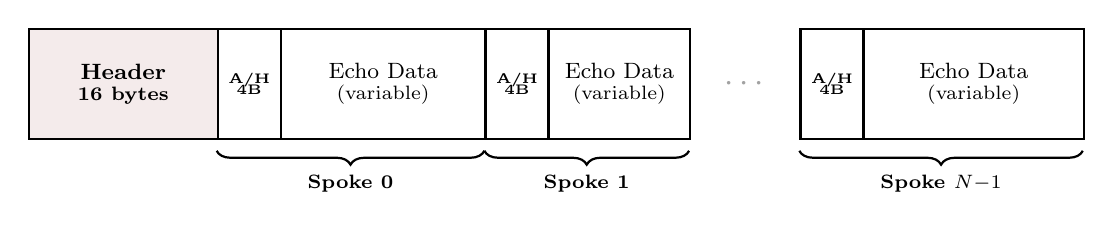
\begin{tikzpicture}[
    block/.style={draw, thick, minimum height=1.4cm, anchor=west, align=center, fill=white, font=\footnotesize},
]

% Header
\node[block, fill=Garnet!8, minimum width=2.4cm, font=\footnotesize\bfseries] (hdr) at (0, 0) {Header\\[-2pt]{\scriptsize 16 bytes}};

% Spoke 0
\node[block, minimum width=0.8cm, font=\tiny\bfseries] (s0h) at (2.4, 0) {A/H\\[-2pt]{\tiny 4B}};
\node[block, minimum width=2.6cm] (s0d) at (3.2, 0) {Echo Data\\[-2pt]{\scriptsize (variable)}};

% Spoke 1
\node[block, minimum width=0.8cm, font=\tiny\bfseries] (s1h) at (5.8, 0) {A/H\\[-2pt]{\tiny 4B}};
\node[block, minimum width=1.8cm] (s1d) at (6.6, 0) {Echo Data\\[-2pt]{\scriptsize (variable)}};

% Dots
\node[font=\large\bfseries, color=FiftyBlack] at (9.1, 0) {$\cdots$};

% Spoke N-1
\node[block, minimum width=0.8cm, font=\tiny\bfseries] (snh) at (9.8, 0) {A/H\\[-2pt]{\tiny 4B}};
\node[block, minimum width=2.8cm] (snd) at (10.6, 0) {Echo Data\\[-2pt]{\scriptsize (variable)}};

% Spoke braces below
\draw[decorate, decoration={brace, amplitude=5pt, mirror}, thick]
    (2.4, -0.85) -- (5.8, -0.85) node[midway, below=5pt, font=\scriptsize\bfseries] {Spoke 0};
\draw[decorate, decoration={brace, amplitude=5pt, mirror}, thick]
    (5.8, -0.85) -- (8.4, -0.85) node[midway, below=5pt, font=\scriptsize\bfseries] {Spoke 1};
\draw[decorate, decoration={brace, amplitude=5pt, mirror}, thick]
    (9.8, -0.85) -- (13.4, -0.85) node[midway, below=5pt, font=\scriptsize\bfseries] {Spoke $N{-}1$};

\end{tikzpicture}
\end{document}
